\documentclass[10pt,twocolumn,letterpaper]{article}

\usepackage{cvpr}
\usepackage{times}
\usepackage{epsfig}
\usepackage{graphicx}
\usepackage{amsmath}
\usepackage{amssymb}
\usepackage{subcaption}

% Include other packages here, before hyperref.

% If you comment hyperref and then uncomment it, you should delete
% egpaper.aux before re-running latex.  (Or just hit 'q' on the first latex
% run, let it finish, and you should be clear).
\usepackage[breaklinks=true,bookmarks=false]{hyperref}

\cvprfinalcopy % *** Uncomment this line for the final submission

\def\cvprPaperID{****} % *** Enter the CVPR Paper ID here
\def\httilde{\mbox{\tt\raisebox{-.5ex}{\symbol{126}}}}

% Pages are numbered in submission mode, and unnumbered in camera-ready
%\ifcvprfinal\pagestyle{empty}\fi
\setcounter{page}{4321}
\begin{document}

%%%%%%%%% TITLE
\title{Generating Audio for Muted Piano-Playing Video Using Deep Learning \newline \newline \textit{Project Milestone}}


\author{XIA Junzhe\\
\tt\small 20493411\\
{\tt\small jxiaaf@connect.ust.hk}
\and
YANG Baichen\\
\tt\small 20493198\\
{\tt\small byangak@connect.ust.hk}
\and
HUANG Zeyu\\
\tt\small 20493631\\
{\tt\small zhuangbi@connect.ust.hk}
}


\maketitle
%\thispagestyle{empty}

%%%%%%%%% BODY TEXT
\section{Introduction}

\subsection{Improved Keyboard Detection}

Among all of the previous work that we have studied, no deep learning based method is used to localize the keyboard in video frame. Instead, all of them used traditional CV method such as Hough Line Transformation, brightness comparison to determine the coordinates of four corners of the piano keyboard. We have first partially reproduced this algorithm.

\begin{figure}[h!]
  \begin{subfigure}{0.24\textwidth}
  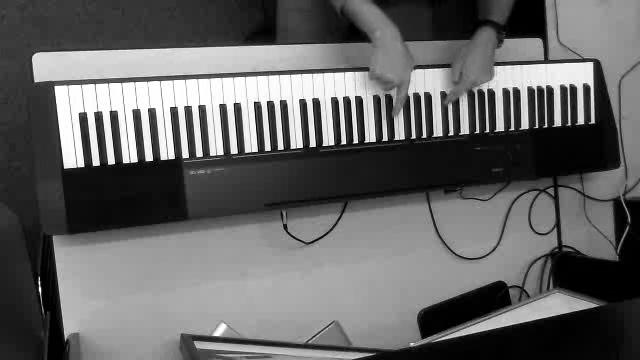
\includegraphics[width=\linewidth]{fig/1.jpg}
  \caption{Original Image in Grayscale} \label{fig:a}
  \end{subfigure}\hspace*{\fill}
  \begin{subfigure}{0.24\textwidth}
  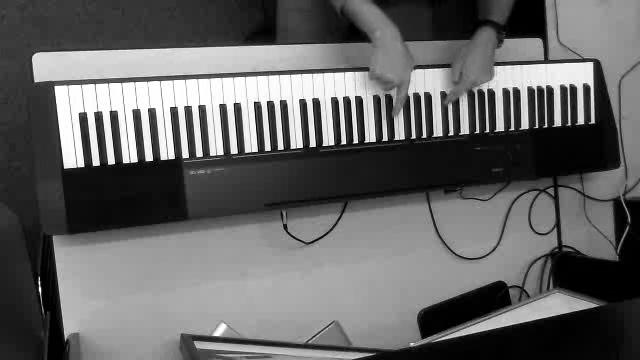
\includegraphics[width=\linewidth]{fig/2.jpg}
  \caption{Gaussian Blurred Image} \label{fig:b}
  \end{subfigure}
  
  \medskip
  \begin{subfigure}{0.24\textwidth}
  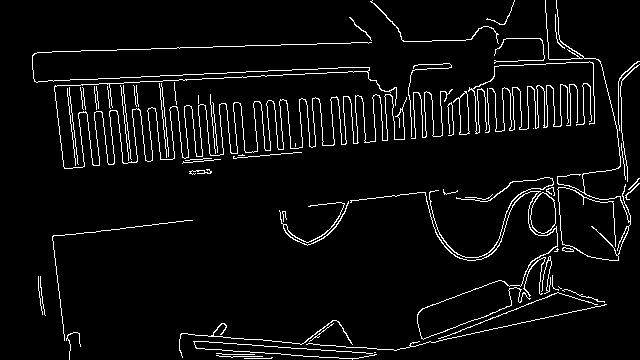
\includegraphics[width=\linewidth]{fig/4.jpg}
  \caption{Canny Edge Detection} \label{fig:c}
  \end{subfigure}\hspace*{\fill}
  \begin{subfigure}{0.24\textwidth}
  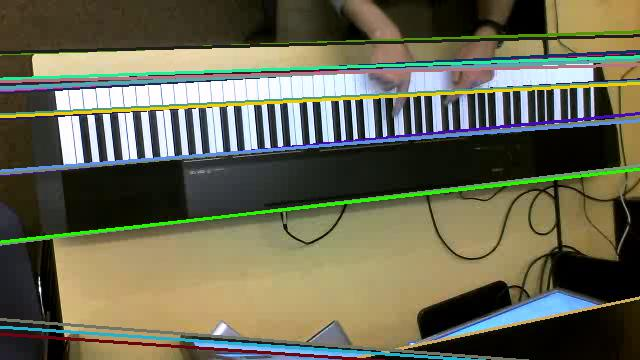
\includegraphics[width=\linewidth]{fig/5.jpg}
  \caption{Hough Line Transformation} \label{fig:d}
  \end{subfigure}
  
  \medskip
  \hspace{2.1cm}
  \begin{subfigure}{0.24\textwidth}
  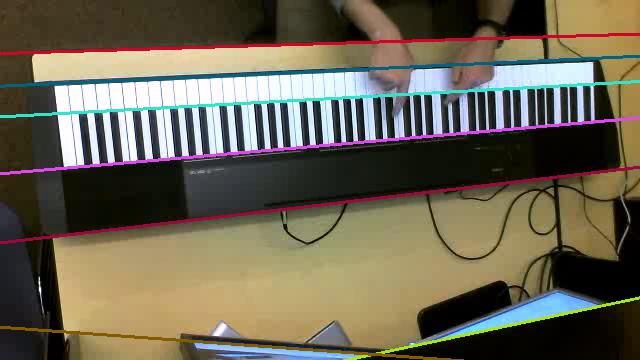
\includegraphics[width=\linewidth]{fig/6.jpg}
  \caption{Prune Repeated Lines} \label{fig:e}
  \end{subfigure}\hspace*{\fill}
  
  \caption{Pipeline of Finding Boundaries of Keyboard} \label{fig:1}
\end{figure}

After pruning repeated lines, some hard-coded method will be used to finally determine the positions of four corners. However, after applying this method to multiple images with different light condition and hand positioning, we found following drawbacks:

\begin{itemize}
  \item To achieve a satisfying performance, several hyperparameters in Hough Line Transformation and Canny Edge Detection needs to be adjusted dramatically in different images.
  \item To accurately determine the corners' coordinates, it is required there is no hands posing above the keyboard. It is hard to guarantee since most of piano videos do not contain such a "empty" frame. In some cases, the camera angle will even change slightly, where the traditional method will fail.
\end{itemize}

Due to the weak robustness of the traditional CV method, we decided to use a convolutional neural network to localize coordinates of four courners of the keyboard. However, we do not have any existing dataset for this task. So we labelled a number of images captured from different piano playing videos, which come from the dataset of a previous work, as well as some videos on the Internet.

\begin{figure}[h!]
  \hspace{2.1cm}
  \begin{subfigure}{0.24\textwidth}
    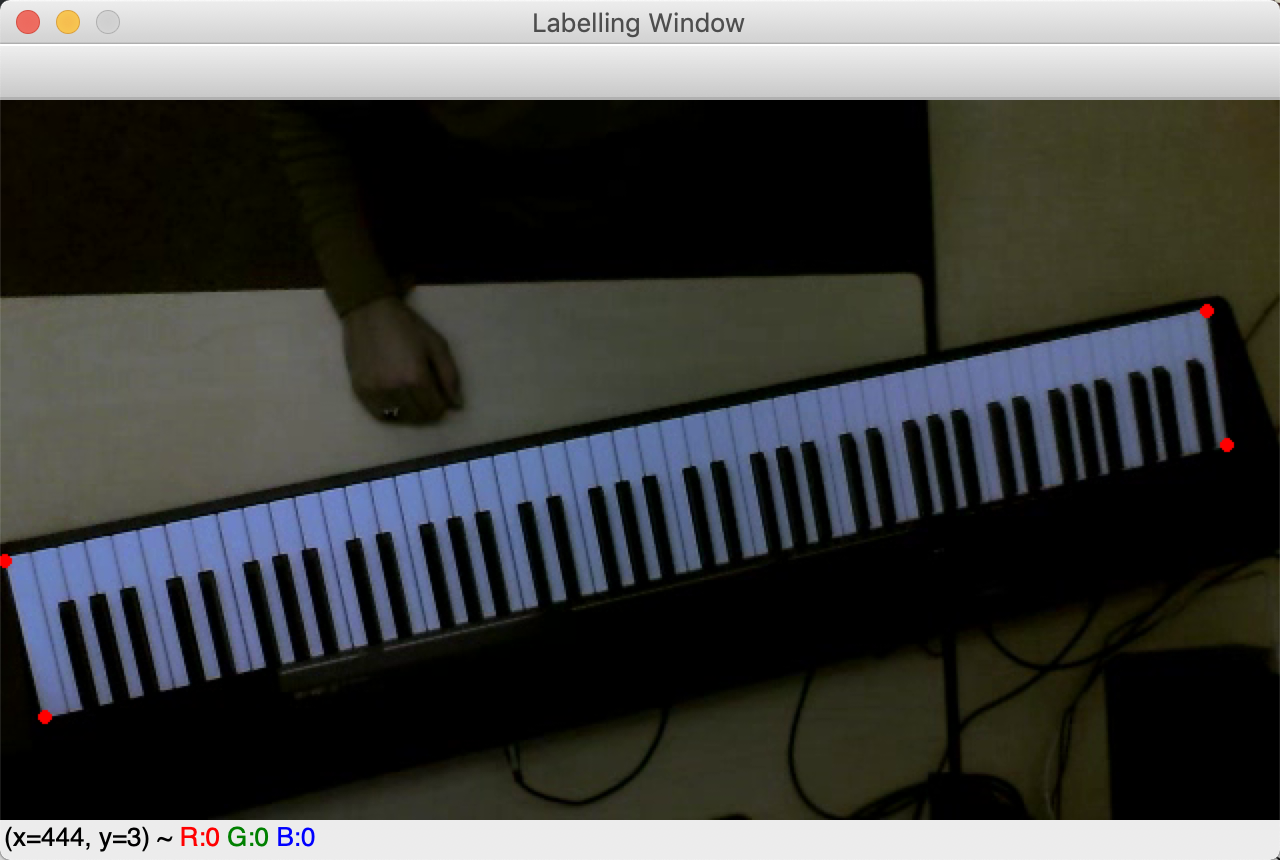
\includegraphics[width=\linewidth]{fig/7.png}      
  \end{subfigure}
  \caption{Labelling Tool}
\end{figure}

To augment this dataset, we will also consider to artificially put keyboard image into some random backgrounds and perform some basic transformation such as flipping and stretching on images present.\\

Parallel to augmentation of the dataset, we have also started to evaluate the performance of several different CNNs on this task.

\section{Future Work}

\subsection{Finalize Keyboard Localization Network}

After experiments and evaluations on different networks, we will be able to decide which CNN that we will use for keyboard localization.

\subsection{Keyboard Separation Algorithm}

After the keyboard can be correctly recognized, we will use perspective transformation to normalize the keyboard in video frame into a preset rectangle structure. Then we will work on an algorithm to extract boundaries of each key, namely, further separate the keyboard into individual keys on this.

\subsection{Train Pressed Key Detection Network}

When individual keys can be localized and normalized, it is feasible for us to perform deep learning on each key to determine their conditions (pressed or not pressed). The quality of the eventual generated music heavily depends on the performace of this network.

\subsection{Velocity Detection Network}

A music piece without emotional variation is rigid and undesired. To detect the velocity information of a key pressing event, we proposed to use a recurrent network to analysis relative frames in order to derive an approximate velocity value of this pressing.

\subsection{Audio Generation}

Upon we can derive all notes information, we need to reconstruct them as a MIDI file. During this process, we may need to smooth out some noisy notes such as those with exceptionally short duration. Besides, it may be necessary to normalize the velocity information we retrieved to avoid unexpected dynamic change.

{\small
\bibliographystyle{ieee}
\bibliography{egbib}
}

\end{document}
